Note: This iteration is slightly longer as it includes the half week between where iteration 10 would have ended and the hand in.

\subsection{Story: Admins can then save the results as csv or xml}
\subsubsection{Analysis - breakdown of tasks}
The most convenient way to save these results would be to convert the data to a csv format, as that can be read by many Spreadsheet programs. After some researching, an extension for Laravel was found that could easily create spreadsheets within a Laravel application\cite{laravel-excel}.

There the list of tasks for this story:
\begin{itemize}
	\item Add route, button and an action for this
	\item Install Laravel spreadsheet converter extension
	\item Pass the formatted answer data into the csv creator
\end{itemize}
\subsubsection{Design}
Due to the way the original answer handling was designed, results are only saved for a session and not for quizzes. This means when a new quiz is run, the results are wiped. This means a good place for the download action would be the quiz admin panel, the one next and previous buttons. This would be an ideal place as it means lecturers can hit download before they end the quiz.

The action itself does not seem to fit onto any of the other controllers, and a new one should be created to handle this function. A sessionController would be the best fit as this action falls under a session and not quizzes so would not be sensible in a quiz controller.

The csv format would be in the form of a single sheet with many rows. The first row would be the question, the second row the answers and the third the number of times the answer was chosen. These three rows would then repeat for each question, so a three question quiz would contain nine rows.
\subsubsection{Implementation}
Setting up the new route, button and controller was a quick task. A new controller was generated, a new route added to the web routing file and a new button added to the admin panel to call this route.

Installing the extension was done with Composer which installed it under the vendor/ folder. It was then added as a Facade\cite{laravel-facades} which allow the quick use and access to the functions it contained. The extension took an array of data and turned that into a spreadsheet of the type specified, in this case a csv. The array is looped over and each item in the array is a row in the sheet. If an item of the array is an arrays itself, then each item within these sub arrays would be a cell within the row. This means the sheet is built from an array of arrays. 

Formatting the arrays was the primary task here. First all the questions from the session were selected, then looped over. Within this loop the question was added as the first row. Then all the answers associated with that question needed to be added. Getting them from the database used a simple Eloquent query. Two arrays needed to be created from this data, an array of the answer text and an array of the number of times these options were submitted. The total times these were submitted had not been calculated so this was done first, looping over the answers and counting the times an answer was given by creating a new array of the answers and times clicked in a key=>value pairing. This array of answer=>answeredNumberTimes could then be looped over and the each key added to the first array, and the values to the second array for the two rows.

The problem here was that the answer text in the database is stored as "answer1" rather than what the student actually clicked. This meant that these answers had to be changed, this was accomplished by using the answer value, like "answer1", as the key in the current question variable and adding this value to a new "keys" array. Another problem was the way multi selection questions were stored, such as "answer1, answer2". This meant adding another extra step to break the string into an array and replacing them with the actual answer values and recombining them into a single string, see appendix \ref{appendix:code} for the function.
\begin{figure}
	\caption{Example of a csv generated}
	\centerline{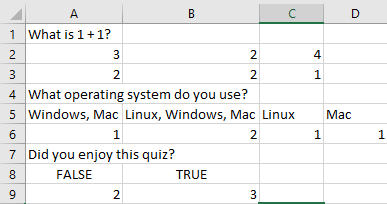
\includegraphics{Chapter2/Iter-10/csv-example}}
	\label{fig:csv-example}
\end{figure}

\subsubsection{Testing}
Not possible to test with Dusk as it is a separate CSV file, but in future a normal PHPUnit test could be written to inspect the array produced and compare it to what is expected.
\newpage

\subsection{Extra implementation based on feedback from admin user tester}
An admin user effectively tested the application whilst using the system to build a quiz that would be used in the user testing. During this, some feedback was received about the application which could be worked on to improve it in small ways.
\subsubsection{Quiz control buttons should be greyed out}
The next and previous buttons on the quiz were changed so that they should be greyed out if the quiz was at the start or end of the quiz. To disable them the "disabled" HTML attribute was added to the buttons. The position and total number of items in the quiz were passed to the page from the controller and could be used to determine whether or not the buttons should be disabled. For these to be disabled when the page loads, some embedded PHP was used to render the buttons with disabled if needed. When the quiz was running, JavaScript was used to add and remove the disabled attribute whenever next or previous was pressed.
\subsubsection{Question creation true/ false changes}
Some JavaScript was used to change the question creation and question edit pages. It was needed for true/ false questions which should be submitted with answer1 as 'True', and answer2 as 'False', with the other fields left blank. The other fields would be ignored when the question was rendered, but allowing them to be filled in could be confusing. So JavaScript was used to hide the other fields, fill the first two with 'True' and 'False', and disable the fields so they could not be edited. This was actually part of the original design for the question creator but was left due to more pressing tasks such as the running of quizzes.
\subsubsection{Cancel button on question edit pages}
Finally, the tester asked if a cancel button could be added, as pressing the back button would work but having a button would probably be better for the users. This was simple a back button placed at the bottom of the edit page.

\subsection{Bugs}
Various bugs were fixed in this final iteration after being found by the admin user. One was a bug concerning the upload time of slides, which took long enough for the PHP execution time to be exceeded. Whilst normally this would require a change to the php.ini file, this was not easily accessible on the server, so a call to the php function, set\_time\_limit() was made to increase this past the default for the function in question. This was a better solution due to it only increasing the limit for the one function, whereas changing the times in the ini file would change the whole system and possibly lead to unintentional side effects.

Another small bug was a "LogicException" found by going to an incorrect url, which is not the standard 404 thrown by an incorrect url. This was caused by a route which had no defined action in the router, something left over from an earlier iteration that ought to have been deleted.

\subsection{User testing}
Used the system in a first year workshop to gather some module feedback for the lecturer and to test the system with real users.

\subsection{Report writing}
A lot of report work in this final iteration, including the restructuring of the iteration and design chapters, writing the design, evaluation, appendices, and generally editing the whole document based on feedback from proof readers.
\newpage